\section{Ziel}
Das Ziel dieses Versuches ist es, anhand der Beugungsfiguren
zweier Einfachspalte die Spaltbreiten zu bestimmen.
Außerdem wird das Beugungsbild eines Doppelspaltes
untersucht. %reicht das?

\section{Theorie}
\label{sec:Theorie}

\subsection{Allgemeines}
Die Beugung des Lichts wird als Abweichung der 
Lichtausbreitung von den Gesetzen der geometrischen Optik 
verstanden. Diese treten auf, wenn Licht auf Öffnungen in 
Schirmen oder auf undurchlässige Hindernisse trifft, die klein
gegenüber dem Strahldurchmesser sind. Die 
Phänomene lassen sich gut beschreiben, wenn die 
Ausbreitung des Lichts als ein Wellenvorgang betrachtet wird. 
Somit gilt zum Beispiel das Huygenssche Prinzip. %

%Fresnel und Fraunhofer
\noindent Es gibt zwei Versuchsanordnungen, die bei Beugungsuntersuchungen 
auftreten können. Dabei werden die Fresnelsche und die 
Fraunhofersche Lichtbeugung unterschieden. Bei der 
Fraunhoferschen Anordnung wird die Lichtquelle ins Unendliche 
verelgt, sodass ein paralleles Lichtbündel mit einer ebenen 
Wellenfront auf die Beugungsebene trifft. Damit wird auch der Aufpunkt 
ins Unendliche  verlegt. Das bedeutet, dass alle Strahlen, die 
in einem Punkt interferieren, unter dem selben Winkel gebeugt 
werden. Dies ist mathematisch einfacher zu behandeln, insofern 
wird diese Anordnung im Folgenden verwendet. 
\newline
Die Länge des zu beugenden Objekts ist groß gegen seine 
Breite $b$. Somit wird das Lichtbündel nur in einer 
Dimension begrenzt.
\newline
%kohärentes Licht, lieber in die Durchführung?
Es wird ein Laser als Lichtquelle benutzt, um kohärentes Licht 
zu erhalten und damit Interferenzerscheinungen möglich zu machen. 
\newline
Aus einer Kombination des Huygensschen Prinzips und der 
Definition des Interferenzprinzips nach Fresnel lässt sich die 
Beugungserscheinung erklären. Das Fresnelsche Prinzip besagt, 
dass jeder Punkt einer Wellenfläche zu gleicher Zeit eine 
Elementarwelle aussendet, die die Form einer Kugelwelle hat. 
Diese neuen Wellen interferieren miteinander. Der 
Schwingungszustand eines beliebigen Punktes ist 
die Superposition aller Elementarwellen, die an dieser Stelle zum 
selben Zeitpunkt eingehen.
\newline
Bei der Messung eines Beugungsbildes lässt sich der Winkel
zwischen Blende und Schirm berechnen durch 
\begin{equation}
    \phi = \arctan (\frac{x}{l}).
    \label{eqn:phi}
\end{equation}
Dabei ist $l$ der Abstand von Blende und Schirm und
$x$ ist der Abstand des Messpunktes zum Hauptmaximum
des Beugungsbildes. %reicht das? phi=0 erwähnen?

\subsection{Beugung am Einzelspalt}
Es wird über die gesamte Spaltbreite integriert, um die 
Amplitude $B$ in Richtung $\phi$ zu bestimmen. Nach Ausführung 
der Integration, Ausklammern eines e-Terms und der Nutzung 
der Euler-Formel, ergibt sich für die Amplitude:
\begin{equation*}
    B(\phi) = A_0 \, b \, \frac{\sin(\frac{\pi \, b \, \sin(\phi)}{\lambda})}{\frac{\pi \, b \, \sin(\phi)}{\lambda}},
\end{equation*}
wobei $b$ die Spaltbreite und $\lambda$ 
die Wellenlänge ist. 
Die Nullstellen der Funktion liegen bei
\begin{equation} 
    sin(\phi_n)= \pm n \frac{\lambda}{b}.
    \label{eqn:nullstellen}
\end{equation}
Dabei ist $n$ eine natürliche Zahl.
Die Amplitude der Lichtwelle lässt sich aufgrund der hohen 
Lichtfrequenz nicht messen. Deshalb kann nur die zeitlich 
gemittelte Intensität bestimmt werden. 
\newline
Diese ergibt sich zu 
\begin{equation}
    I(\phi) \propto B(\phi)^2 = A^{2}_0 \, b^2 \, \left(\frac{\lambda}{\pi \, b \, sin(\phi)} \right)^2 \cdot sin \left(\frac{\pi \, b \, sin(\phi)}{\lambda}\right).
    \label{eqn:intensität}
\end{equation}
Eine theoretische Intensitätsverteilung für den Einzelspalt
ist in Abb. \ref{fig:} zu sehen.
\begin{figure}
    \centering
    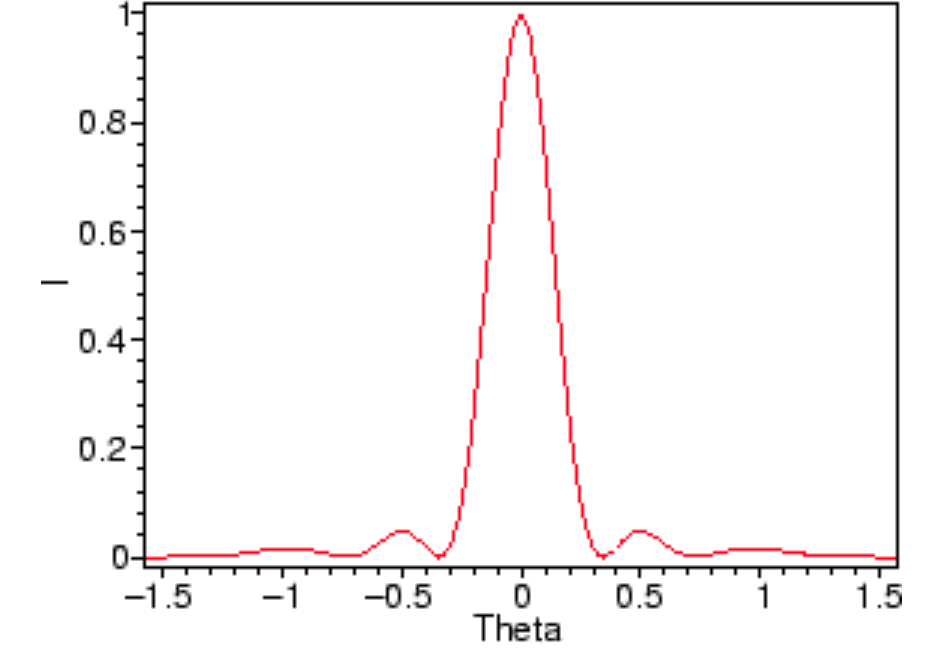
\includegraphics[width=5cm, height=4cm]{build/Einzelspalt.png}
    \caption{Die Intensitätsverteilung für einen Einzelspalt. \cite{einzel}}
    \label{fig:einzel}
\end{figure}

\subsection{Beugung am Doppelspalt}
Analog dazu lassen sich auch Nullstellen der Amplitude und 
die gemittelte Intensität bei der Beugung des Lichts am 
Doppelspalt bestimmen.
Die Nullstellen liegen bei 
\begin{equation}
    \phi(k) = arcsin \left(\frac{2k+1}{2s}\cdot \lambda \right).
    \label{eqn:doppelns}
\end{equation}
Dabei ist $s$ die Breite des Spalts zusammen mit
dem Abstand zwischen den beiden Spalten.
\newline
Die Intensität ergibt sich zu 
\begin{equation}
    I(\phi) \propto B(\phi)^2 =4 \, cos^2 \left(\frac{\pi \, s \, sin(\phi)}{\lambda} \right)\cdot \left(\frac{\lambda}{\pi \, b \, sin(\phi)} \right)^2 \cdot sin^2 \left(\frac{\pi \, b \, sin(\phi)}{\lambda}\right).
    \label{eqn:doppelintensität}
\end{equation}
Eine theoretische Intensitätsverteilung für den Doppelspalt
ist in Abb. \ref{fig:doppel} zu sehen.
\begin{figure}
    \centering
    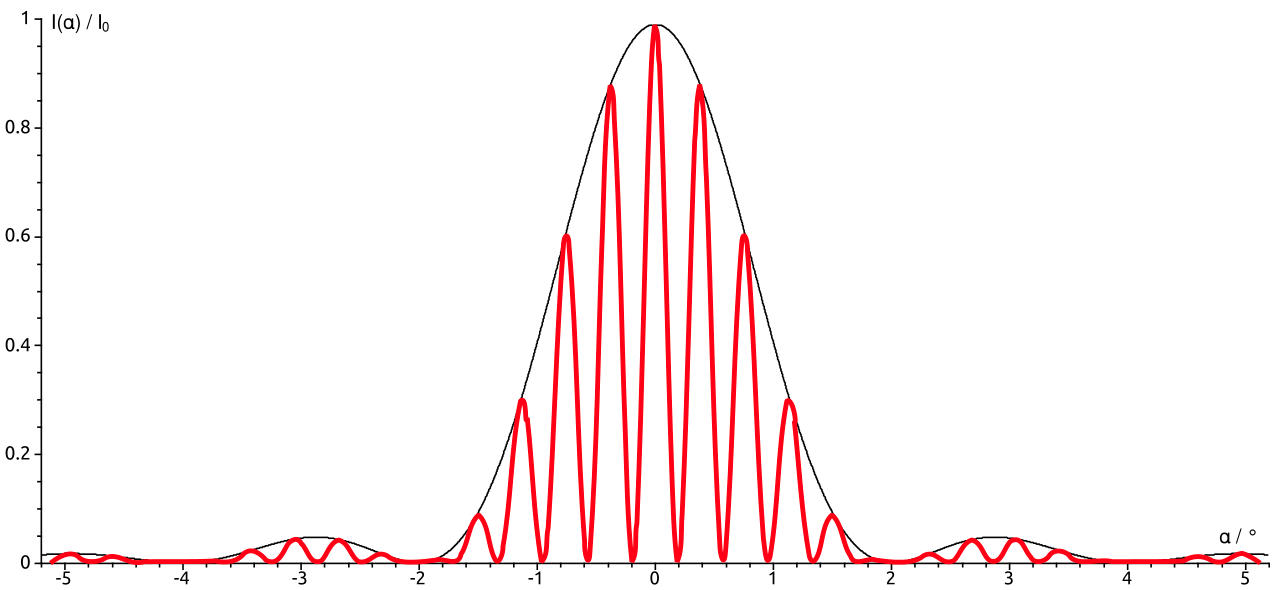
\includegraphics[width=10cm, height=5cm]{build/Doppelspalt.png}
    \caption{Die Intensitätsverteilung für den Doppelspalt. \cite{doppel}}
\end{figure}